\chapter{Pression atmosphérique et météo}\label{ch:g5:air-pressure-weather}

Tu vis au fond d'un océan --- un océan d'\omterm{def:g2:air-around-us:air}{air}, profond de centaines de
kilomètres, dont tout le \omterm{def:g4:weight-and-mass:weight}{poids} repose sur tes épaules. Pourquoi ne
t'écrase-t-il pas~? Pourquoi ne le sens-tu même pas~? Et quel rapport
tout cela a-t-il avec le temps qu'il fera demain~? L'\omterm{def:g2:air-around-us:air}{air}, notre vieil
ami invisible, a encore un grand secret à livrer.

\section{L'air a un poids}

\begin{example}[Peser l'invisible]\label{ex:g5:air-pressure-weather:weighing}
On pose un ballon de football bien gonflé sur une \omterm{def:g3:levers-and-scales:scale}{balance} de
précision et on l'équilibre exactement. Puis on ouvre sa valve et
l'\omterm{def:g2:air-around-us:air}{air} en trop s'échappe en sifflant --- même ballon, même valve, tout
pareil, moins un peu d'\omterm{def:g2:air-around-us:air}{air}. De retour sur la \omterm{def:g3:levers-and-scales:scale}{balance}~: le ballon
dégonflé est \emph{plus léger}. La différence est le \omterm{def:g4:weight-and-mass:weight}{poids} de l'\omterm{def:g2:air-around-us:air}{air}
échappé. L'\omterm{def:g2:air-around-us:air}{air} est de la matière, la matière a une \omterm{def:g3:measuring-mass:mass}{masse}, et la \omterm{def:g3:measuring-mass:mass}{masse}
est tirée vers le bas par la Terre~: l'océan au-dessus de nous est
lourd.
\end{example}

\begin{definition}[L'atmosphère et sa pression]\label{def:g5:air-pressure-weather:pressure}
L'\emph{atmosphère}\index{atmosphère} est la couche profonde d'\omterm{def:g2:air-around-us:air}{air}
enveloppant la Terre tout entière. Son \omterm{def:g4:weight-and-mass:weight}{poids} comprime l'\omterm{def:g2:air-around-us:air}{air} du
fond --- là où nous vivons --- et l'\omterm{def:g2:air-around-us:air}{air} comprimé appuie fortement sur
chaque surface qu'il touche. Cet appui s'appelle la \emph{pression
atmosphérique}\index{pression atmosphérique}.
\end{definition}

\begin{proposition}[L'appui de tous les côtés]\label{prop:g5:air-pressure-weather:allsides}
La \omterm{def:g5:air-pressure-weather:pressure}{pression atmosphérique} appuie sur chaque surface dans
\emph{toutes} les directions --- vers le bas sur les tables, de côté
sur les murs, et même \emph{vers le haut} sur les plafonds et les
paumes. Et elle est puissante~: sur une surface grande comme ta
paume, l'\omterm{def:g2:air-around-us:air}{air} appuie à peu près aussi fort que le \omterm{def:g4:weight-and-mass:weight}{poids} d'une grosse
valise pleine. Nous ne le remarquons jamais, parce que les appuis
s'équilibrent~: l'\omterm{def:g2:air-around-us:air}{air} qui est en nous et derrière chaque surface
repousse tout aussi fort.
\end{proposition}

\begin{method}[La carte qui retient l'eau]\label{met:g5:air-pressure-weather:card}
L'appui vers le haut de l'\omterm{def:g2:air-around-us:air}{air}, pris la main dans le sac (à faire
au-dessus de l'évier)~:
\begin{enumerate}
  \item remplir un verre d'eau jusqu'au bord~;
  \item poser à plat dessus une carte rigide et lisse, qui touche
        l'eau tout autour~;
  \item maintenir la carte en place, retourner le verre exactement
        à l'envers, puis lâcher doucement la carte.
\end{enumerate}
La carte tient --- en retenant tout le contenu du verre. Le \omterm{def:g4:weight-and-mass:weight}{poids} de
l'eau appuie sur la carte vers le bas, mais l'\omterm{def:g5:air-pressure-weather:pressure}{atmosphère} appuie
\emph{vers le haut} plus fort encore. Tu viens de voir l'appui de la
valise, par en dessous.
\end{method}

\begin{omfigure}
\begin{tikzpicture}[scale=0.85]
  \draw[thick] (4.4,1.2) -- (4.4,3.6) (6.6,1.2) -- (6.6,3.6);
  \draw[thick] (4.4,3.6) -- (6.6,3.6);
  \fill[omDef, opacity=0.25] (4.4,1.25) rectangle (6.6,3.55);
  \draw[very thick, omMeth] (4.25,1.2) -- (6.75,1.2);
  \node[right, font=\small, omMeth] at (6.9,1.2) {la carte};
  \draw[-Stealth, thick, omDef] (5.0,2.9) -- (5.0,2.2);
  \draw[-Stealth, thick, omDef] (6.0,2.9) -- (6.0,2.2);
  \node[above, font=\small, omDef] at (5.5,3.65)
    {l'eau appuie vers le bas};
  \foreach \x in {4.7,5.5,6.3} {
    \draw[-Stealth, very thick, omThm] (\x,0.15) -- (\x,0.95);
  }
  \node[below, font=\small, omThm] at (5.5,-0.05)
    {l'atmosphère appuie vers le haut --- plus fort};
\end{tikzpicture}

{\small Le verre retourné~: l'appui de l'\omterm{def:g2:air-around-us:air}{air} vers le haut sur la
carte l'emporte sur le \omterm{def:g4:weight-and-mass:weight}{poids} de l'eau. L'océan invisible est
puissant.}
\end{omfigure}

\section{Des machines mues par l'atmosphère}

\begin{example}[La paille]\label{ex:g5:air-pressure-weather:straw}
Tu crois aspirer le jus dans la paille. En vérité, on ne peut pas
tirer un \omterm{def:g3:solids-liquids-gases:liquid}{liquide} du tout --- essaie donc de tirer de l'eau avec les
doigts~! Ce que tu fais réellement, c'est aspirer l'\emph{\omterm{def:g2:air-around-us:air}{air}} hors
de la paille. L'\omterm{def:g2:air-around-us:air}{air} parti de l'intérieur, l'\omterm{def:g5:air-pressure-weather:pressure}{atmosphère} qui appuie sur
le jus dans le verre pousse le jus dans la paille vide jusqu'à ta
bouche. Chaque gorgée est l'\omterm{def:g5:air-pressure-weather:pressure}{atmosphère} qui fait le travail~; toi, tu
ne fais que dégager la route.
\end{example}

\begin{example}[Ventouses et bouteilles écrasées]\label{ex:g5:air-pressure-weather:suction}
La ventouse en caoutchouc du crochet de salle de bain est écrasée
contre le carrelage, ce qui chasse l'\omterm{def:g2:air-around-us:air}{air} de dessous~: l'\omterm{def:g5:air-pressure-weather:pressure}{atmosphère}
plaque alors la ventouse contre le mur sans que rien, derrière, ne
repousse --- épinglée par le ciel lui-même. Et visse le bouchon sur
une bouteille en plastique vide, tout en haut d'une montagne, puis
redescends dans la vallée~: la bouteille se froisse comme écrasée par
une main fantôme. Il y a plus d'\omterm{def:g2:air-around-us:air}{air} qui appuie dehors que d'\omterm{def:g2:air-around-us:air}{air} de
montagne, raréfié, enfermé dedans --- l'\omterm{def:g5:air-pressure-weather:pressure}{atmosphère} gagne, et la
bouteille se plie.
\end{example}

\begin{example}[De plus en plus rare avec
l'altitude]\label{ex:g5:air-pressure-weather:height}
Monte, et tu laisses une partie de l'océan au-dessous de toi~: moins
d'\omterm{def:g2:air-around-us:air}{air} au-dessus signifie un appui plus faible. Tes oreilles se
bouchent dans un téléphérique rapide, quand la pression extérieure
change~; les alpinistes suffoquent dans un \omterm{def:g2:air-around-us:air}{air} devenu rare. Et voici
que le mystère du thé de montagne de l'an dernier se rend~: comme
l'\omterm{def:g5:air-pressure-weather:pressure}{atmosphère} appuie moins sur l'eau, l'ébullition vient plus
facilement --- l'eau, sur les grands sommets, bout bien au-dessous de
\qty{100}{\celsius}, trop tiède pour une bonne infusion.
\end{example}

\begin{omfigure}
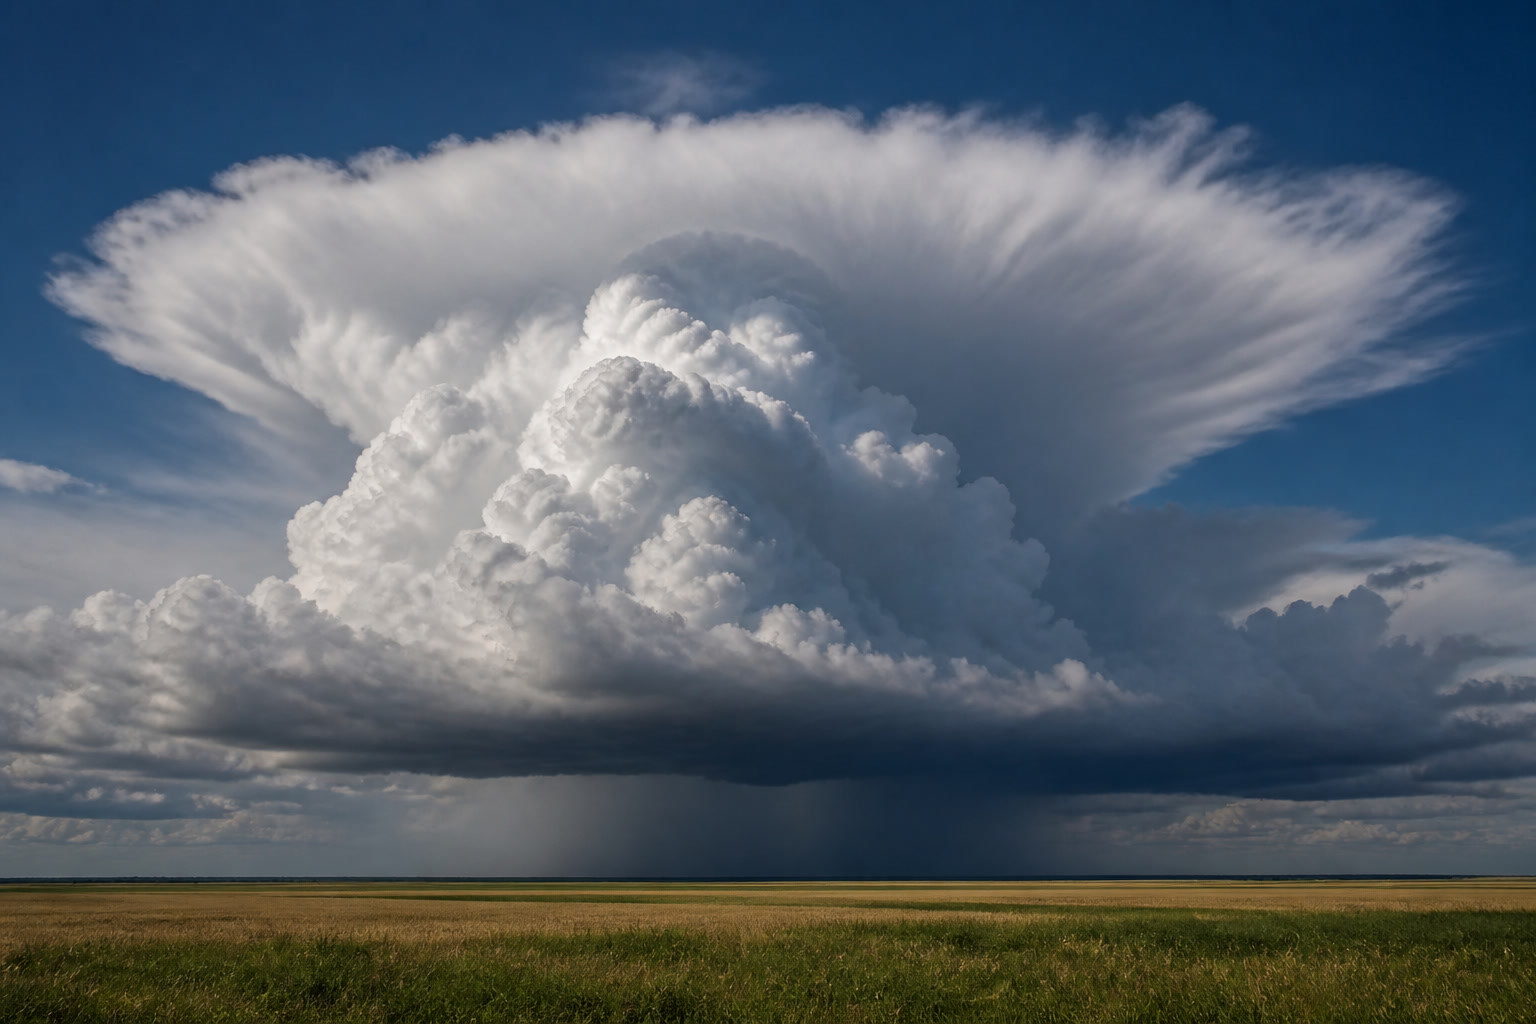
\includegraphics[width=0.58\linewidth]{images/book1/ai/g5-weather-storm.jpg}

{\small Un nuage d'orage dressé au-dessus des champs~: la météo, c'est l'\omterm{def:g5:air-pressure-weather:pressure}{atmosphère} en mouvement.}
\end{omfigure}

\section{Le baromètre et le temps qu'il fera}

\begin{definition}[Baromètre]\label{def:g5:air-pressure-weather:barometer}
Un \emph{baromètre}\index{baromètre} est l'instrument qui mesure la
\omterm{def:g5:air-pressure-weather:pressure}{pression atmosphérique} --- un membre de plus dans notre famille de
juges honnêtes, aux côtés du \omterm{def:g3:temperature-thermometers:temperature}{thermomètre} et de la \omterm{def:g3:levers-and-scales:scale}{balance}. Son
aiguille monte quand l'\omterm{def:g5:air-pressure-weather:pressure}{atmosphère} au-dessus appuie plus fort, et
descend quand l'appui s'allège.
\end{definition}

\begin{proposition}[La pression parle de demain]\label{prop:g5:air-pressure-weather:weather}
La pression de l'\omterm{def:g5:air-pressure-weather:pressure}{atmosphère} ne tient pas en place~: un \omterm{def:g2:air-around-us:air}{air} lourd qui
descend apporte un ciel calme et clair~; un \omterm{def:g2:air-around-us:air}{air} léger qui monte
invite les nuages et la pluie. Le \omterm{def:g5:air-pressure-weather:barometer}{baromètre} est donc une diseuse de
bonne aventure, modeste et honnête~: une pression \emph{stable ou en
hausse} promet du beau temps~; une pression \emph{en baisse} annonce
l'arrivée des nuages~; une \emph{chute rapide} signifie qu'une
tempête est peut-être en route.
\end{proposition}

\begin{omfigure}
\begin{tikzpicture}[scale=0.85]
  \draw[thick] (2.2,1.7) circle (1.5);
  \foreach \a/\t in {150/{}, 120/{}, 90/{}, 60/{}, 30/{}} {
    \draw (2.2,1.7) ++(\a:1.3) -- ++(\a:0.18);
  }
  \node[font=\footnotesize] at (1.1,2.6) {pluie};
  \node[font=\footnotesize] at (2.2,3.0) {variable};
  \node[font=\footnotesize] at (3.4,2.6) {beau};
  \draw[-Stealth, very thick, omThm] (2.2,1.7) -- ++(55:1.1);
  \fill (2.2,1.7) circle (2pt);
  \node[below, font=\small] at (2.2,-0.05)
    {un baromètre de maison~: l'aiguille penche vers le beau};
  \node[right, font=\small, align=left] at (5.4,2.5)
    {aiguille qui monte~: ciel dégagé en vue};
  \node[right, font=\small, align=left] at (5.4,1.7)
    {aiguille qui descend~: les nuages arrivent};
  \node[right, font=\small, align=left] at (5.4,0.9)
    {chute rapide~: aux abris --- tempête};
\end{tikzpicture}

{\small Lire un \omterm{def:g5:air-pressure-weather:barometer}{baromètre}~: moins l'endroit où se tient l'aiguille
que le sens dans lequel elle se déplace --- l'\omterm{def:g5:air-pressure-weather:pressure}{atmosphère} annonce ses
intentions.}
\end{omfigure}

\begin{remark}[Les A et les D de la carte
météo]\label{rem:g5:air-pressure-weather:map}
Le bulletin météo de ce soir montrera de grands tourbillons marqués A
et D~: des zones de haute et de basse pression qui dérivent sur la
carte comme de lentes baleines. L'\omterm{def:g2:air-around-us:air}{air} s'écoule sans cesse des zones
lourdes marquées A (les anticyclones) vers les zones légères marquées
D (les dépressions) --- et cet écoulement \emph{est le \omterm{def:g2:air-around-us:wind}{vent}}. Un seul
chapitre, trois vieilles connaissances expliquées~: la prévision du
\omterm{def:g5:air-pressure-weather:barometer}{baromètre}, l'origine du \omterm{def:g2:air-around-us:wind}{vent}, et la raison pour laquelle tes oreilles
savent quand le temps est sur le point de tourner.
\end{remark}

\section{Exercices}

\begin{exercise}[$\star$]\label{exo:g5:air-pressure-weather:1}
Comment l'expérience du ballon de football montre-t-elle que l'\omterm{def:g2:air-around-us:air}{air} a
un \omterm{def:g4:weight-and-mass:weight}{poids}~? Que compare-t-on exactement~?
\end{exercise}

\begin{exercise}[$\star$]\label{exo:g5:air-pressure-weather:2}
Qu'est-ce que la \omterm{def:g5:air-pressure-weather:pressure}{pression atmosphérique}, et d'où vient-elle~? Dans
quelles directions appuie-t-elle~?
\end{exercise}

\begin{exercise}[$\star$]\label{exo:g5:air-pressure-weather:3}
L'\omterm{def:g5:air-pressure-weather:pressure}{atmosphère} appuie sur ta paume à peu près aussi fort que pèse une
valise pleine --- et pourtant tu ne sens rien. Pourquoi~?
\end{exercise}

\begin{exercise}[$\star$]\label{exo:g5:air-pressure-weather:4}
Dans le tour de la carte, deux appuis se disputent la carte. Nomme-les,
et dis lequel l'emporte.
\end{exercise}

\begin{exercise}[$\star$]\label{exo:g5:air-pressure-weather:5}
«~J'aspire le jus dans la paille.~» Corrige cette phrase~: qu'est-ce
que tu enlèves réellement, et qui fait le travail de soulever~?
\end{exercise}

\begin{exercise}[$\star$]\label{exo:g5:air-pressure-weather:6}
Pourquoi une ventouse adhère-t-elle au carrelage~? Qu'a-t-on chassé,
et qu'est-ce qui maintient la ventouse~?
\end{exercise}

\begin{exercise}[$\star$]\label{exo:g5:air-pressure-weather:7}
Qu'arrive-t-il à la \omterm{def:g5:air-pressure-weather:pressure}{pression atmosphérique} quand on grimpe une
montagne, et pourquoi~? Donne-en deux signes qu'un voyageur peut
remarquer.
\end{exercise}

\begin{exercise}[$\star$]\label{exo:g5:air-pressure-weather:8}
Que mesure un \omterm{def:g5:air-pressure-weather:barometer}{baromètre}~? Le tien descend rapidement depuis le
petit-déjeuner --- à quoi doivent s'attendre les projets de
pique-nique~?
\end{exercise}

\begin{exercise}[$\star\star$]\label{exo:g5:air-pressure-weather:9}
La bouteille fermée s'est froissée pendant la descente de la
montagne. Explique le froissement avec les appuis intérieur et
extérieur --- et prédis~: qu'arriverait-il, au contraire, à une
bouteille fermée dans la vallée puis emportée \emph{vers le haut}~?
\end{exercise}

\begin{exercise}[$\star\star$]\label{exo:g5:air-pressure-weather:10}
D'où vient le \omterm{def:g2:air-around-us:wind}{vent}, d'après les tourbillons A et D de la carte
météo~? Relie cela à la plus ancienne définition de ce livre~: le
\omterm{def:g2:air-around-us:wind}{vent} est de l'\omterm{def:g2:air-around-us:air}{air} en mouvement --- mis en mouvement par quoi~?
\end{exercise}

\begin{exercise}[$\star\star$]\label{exo:g5:air-pressure-weather:11}
Les alpinistes se plaignent que, sur les grands sommets, le thé
n'infuse jamais fort et que les pâtes restent dures quelle que soit
la \omterm{def:g2:measuring-time:duration}{durée} de l'ébullition. Rassemble l'explication complète sur deux
années~: que fait l'\omterm{def:g5:air-pressure-weather:pressure}{atmosphère} raréfiée à la \omterm{def:g4:changes-of-state:boiling-point}{température
d'ébullition}, et pourquoi bouillir plus longtemps n'y change-t-il
rien~? (Deux propositions, dont une de l'an dernier, closent
l'affaire.)
\end{exercise}
